%%%%%%%%%%%%%%%%%%%%%%%%%%%%%%%%%%%%%%%%%%%%%%%%%%%%%%%%%%%%%%%%%%%
% Cocca, Giordano,  Vassio
% from November 2017
%%%%%%%%%%%%%%%%%%%%%%%%%%%%%%%%%%%%%%%%%%%%%%%%%%%%%%%%%%%%%%%%%%%


\documentclass[conference]{IEEEtran}
\IEEEoverridecommandlockouts
% The preceding line is only needed to identify funding in the first footnote. If that is unneeded, please comment it out.
\usepackage{cite}
\usepackage{amsmath,amssymb,amsfonts}
\usepackage{algorithmic}
\usepackage{graphicx}
\usepackage{textcomp}
\usepackage{hyperref}

\usepackage{graphicx}
%\usepackage{subfigure}
\usepackage{caption}
\usepackage{subcaption}

\usepackage{xcolor}

%encoding
%--------------------------------------
\usepackage[utf8]{inputenc}
\usepackage[T1]{fontenc}
%--------------------------------------
 
%Portuguese-specific commands
%--------------------------------------
\usepackage[portuguese]{babel}
%--------------------------------------
 
%Hyphenation rules
%--------------------------------------
\usepackage{hyphenat}
\hyphenation{mate-mática recu-perar}
%--------------------------------------

\usepackage{multirow}


\def\BibTeX{{\rm B\kern-.05em{\sc i\kern-.025em b}\kern-.08em
    T\kern-.1667em\lower.7ex\hbox{E}\kern-.125emX}}
\usepackage{url}
\usepackage{verbatim}


\usepackage[ruled]{algorithm2e} % For algorithms
%\usepackage{subfigure}
%\ProvidesPackage{xstring}[\xstringdate\space\space v\xstringversion\space\space String manipulations (C Tellechea)]
%\usepackage{booktabs} % For formal tables

\newcommand{\tool}{\textit{UMAP}\xspace}

\DeclareMathOperator*{\argmax}{arg\,max}
\DeclareMathOperator*{\argmin}{arg\,min}

% To comment in the paper
\usepackage{color}
\newcommand{\lu}[1]{{\color{cyan}{[luca: #1]}}}
\newcommand{\mc}[1]{{\color{green}{[mike: #1]}}}
\newcommand{\mm}[1]{{\color{red}{[mellia: #1]}}}
\newcommand{\dg}[1]{{\color{orange}{[DG: #1]}}}

%% Document starts
\begin{document}


\title{Free Floating Electric Car Sharing:\\A Big Data approach for System Design
% * <michelecocca.mc@gmail.com> 2018-08-15T18:37:09.766Z:
%
% > loati
%
% ^.
\thanks{The work is supported by General Motors Powertrain grant, and by the SmartData@PoliTO centre.}
}

\author{
\IEEEauthorblockN{Michele Cocca}
\IEEEauthorblockA{%\textit{Department of Electronics and Telecommunications} \\
\textit{Politecnico di Torino, Italy}\\
%Turin, Italy\\
michele.cocca@polito.it}
\and
\IEEEauthorblockN{Danilo Giordano}
\IEEEauthorblockA{%\textit{Department of Electronics and Telecommunications} \\
\textit{Politecnico di Torino, Italy}\\
%Turin, Italy\\
danilo.giordano@polito.it}
\and
\IEEEauthorblockN{Marco Mellia}
\IEEEauthorblockA{%\textit{Department of Electronics and Telecommunications} \\
\textit{Politecnico di Torino, Italy}\\
%Turin, Italy\\
marco.mellia@polito.it}
\and
%\hspace{50pt}
\IEEEauthorblockN{Luca Vassio}
\IEEEauthorblockA{%\textit{Department of Electronics and Telecommunications} \\
\textit{Politecnico di Torino, Italy}\\
%Turin, Italy\\
luca.vassio@polito.it}
}

\maketitle

\input{abstract}


\begin{IEEEkeywords}
car sharing, electric vehicle, data driven optimization, big data, charging station, free floating.
\end{IEEEkeywords}


\input{intro}
\input{related_work}
\input{Data}
\input{Modelling}
\input{PlacementResults}
\input{ReturnResults}
\input{PolesResults}
 \input{Conclusion}



\bibliographystyle{IEEEtran}
\bibliography{paper}

\section*{Biographies}

\begin{IEEEbiography}[{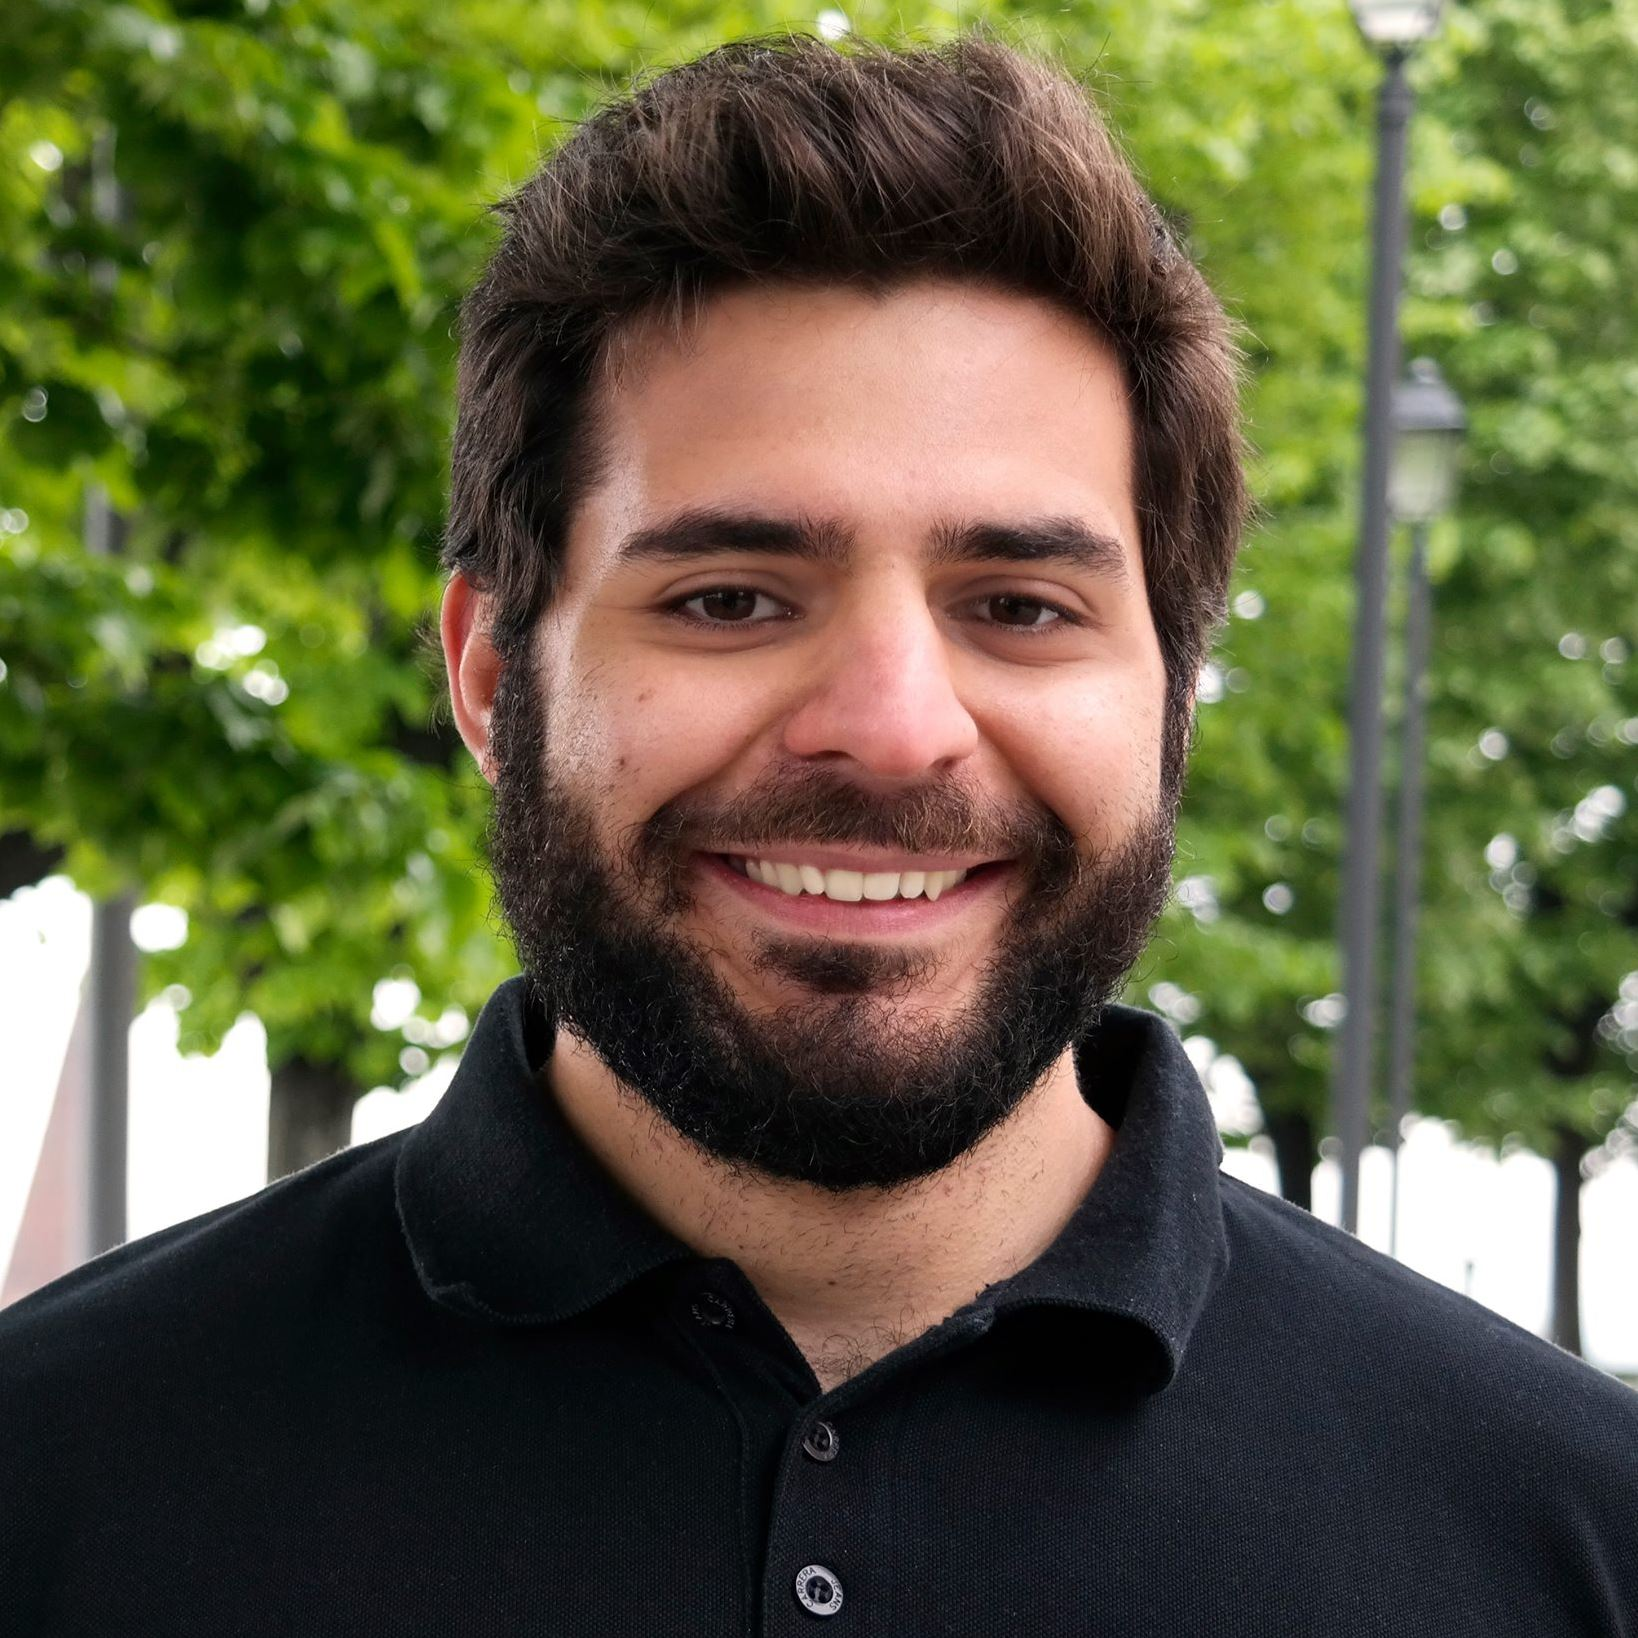
\includegraphics[width=1in,height=1.25in,clip,keepaspectratio]{bios/michele.jpg}}] {Michele Cocca} is a Ph.D. student since 2017 in the Department of Electronics and Telecommunications at Politecnico di Torino, Italy. His research is focused on data analysis of smart transportation systems, with particular attention on forecasting and simulating people interaction with electric shared vehicles. In August 2018 he moved for a visiting period of 18 months to Computer Science Department at Universidade Federal de Minas Gerais (UFMG), Belo Horizonte, Brazil.
\end{IEEEbiography}


\begin{IEEEbiography}[{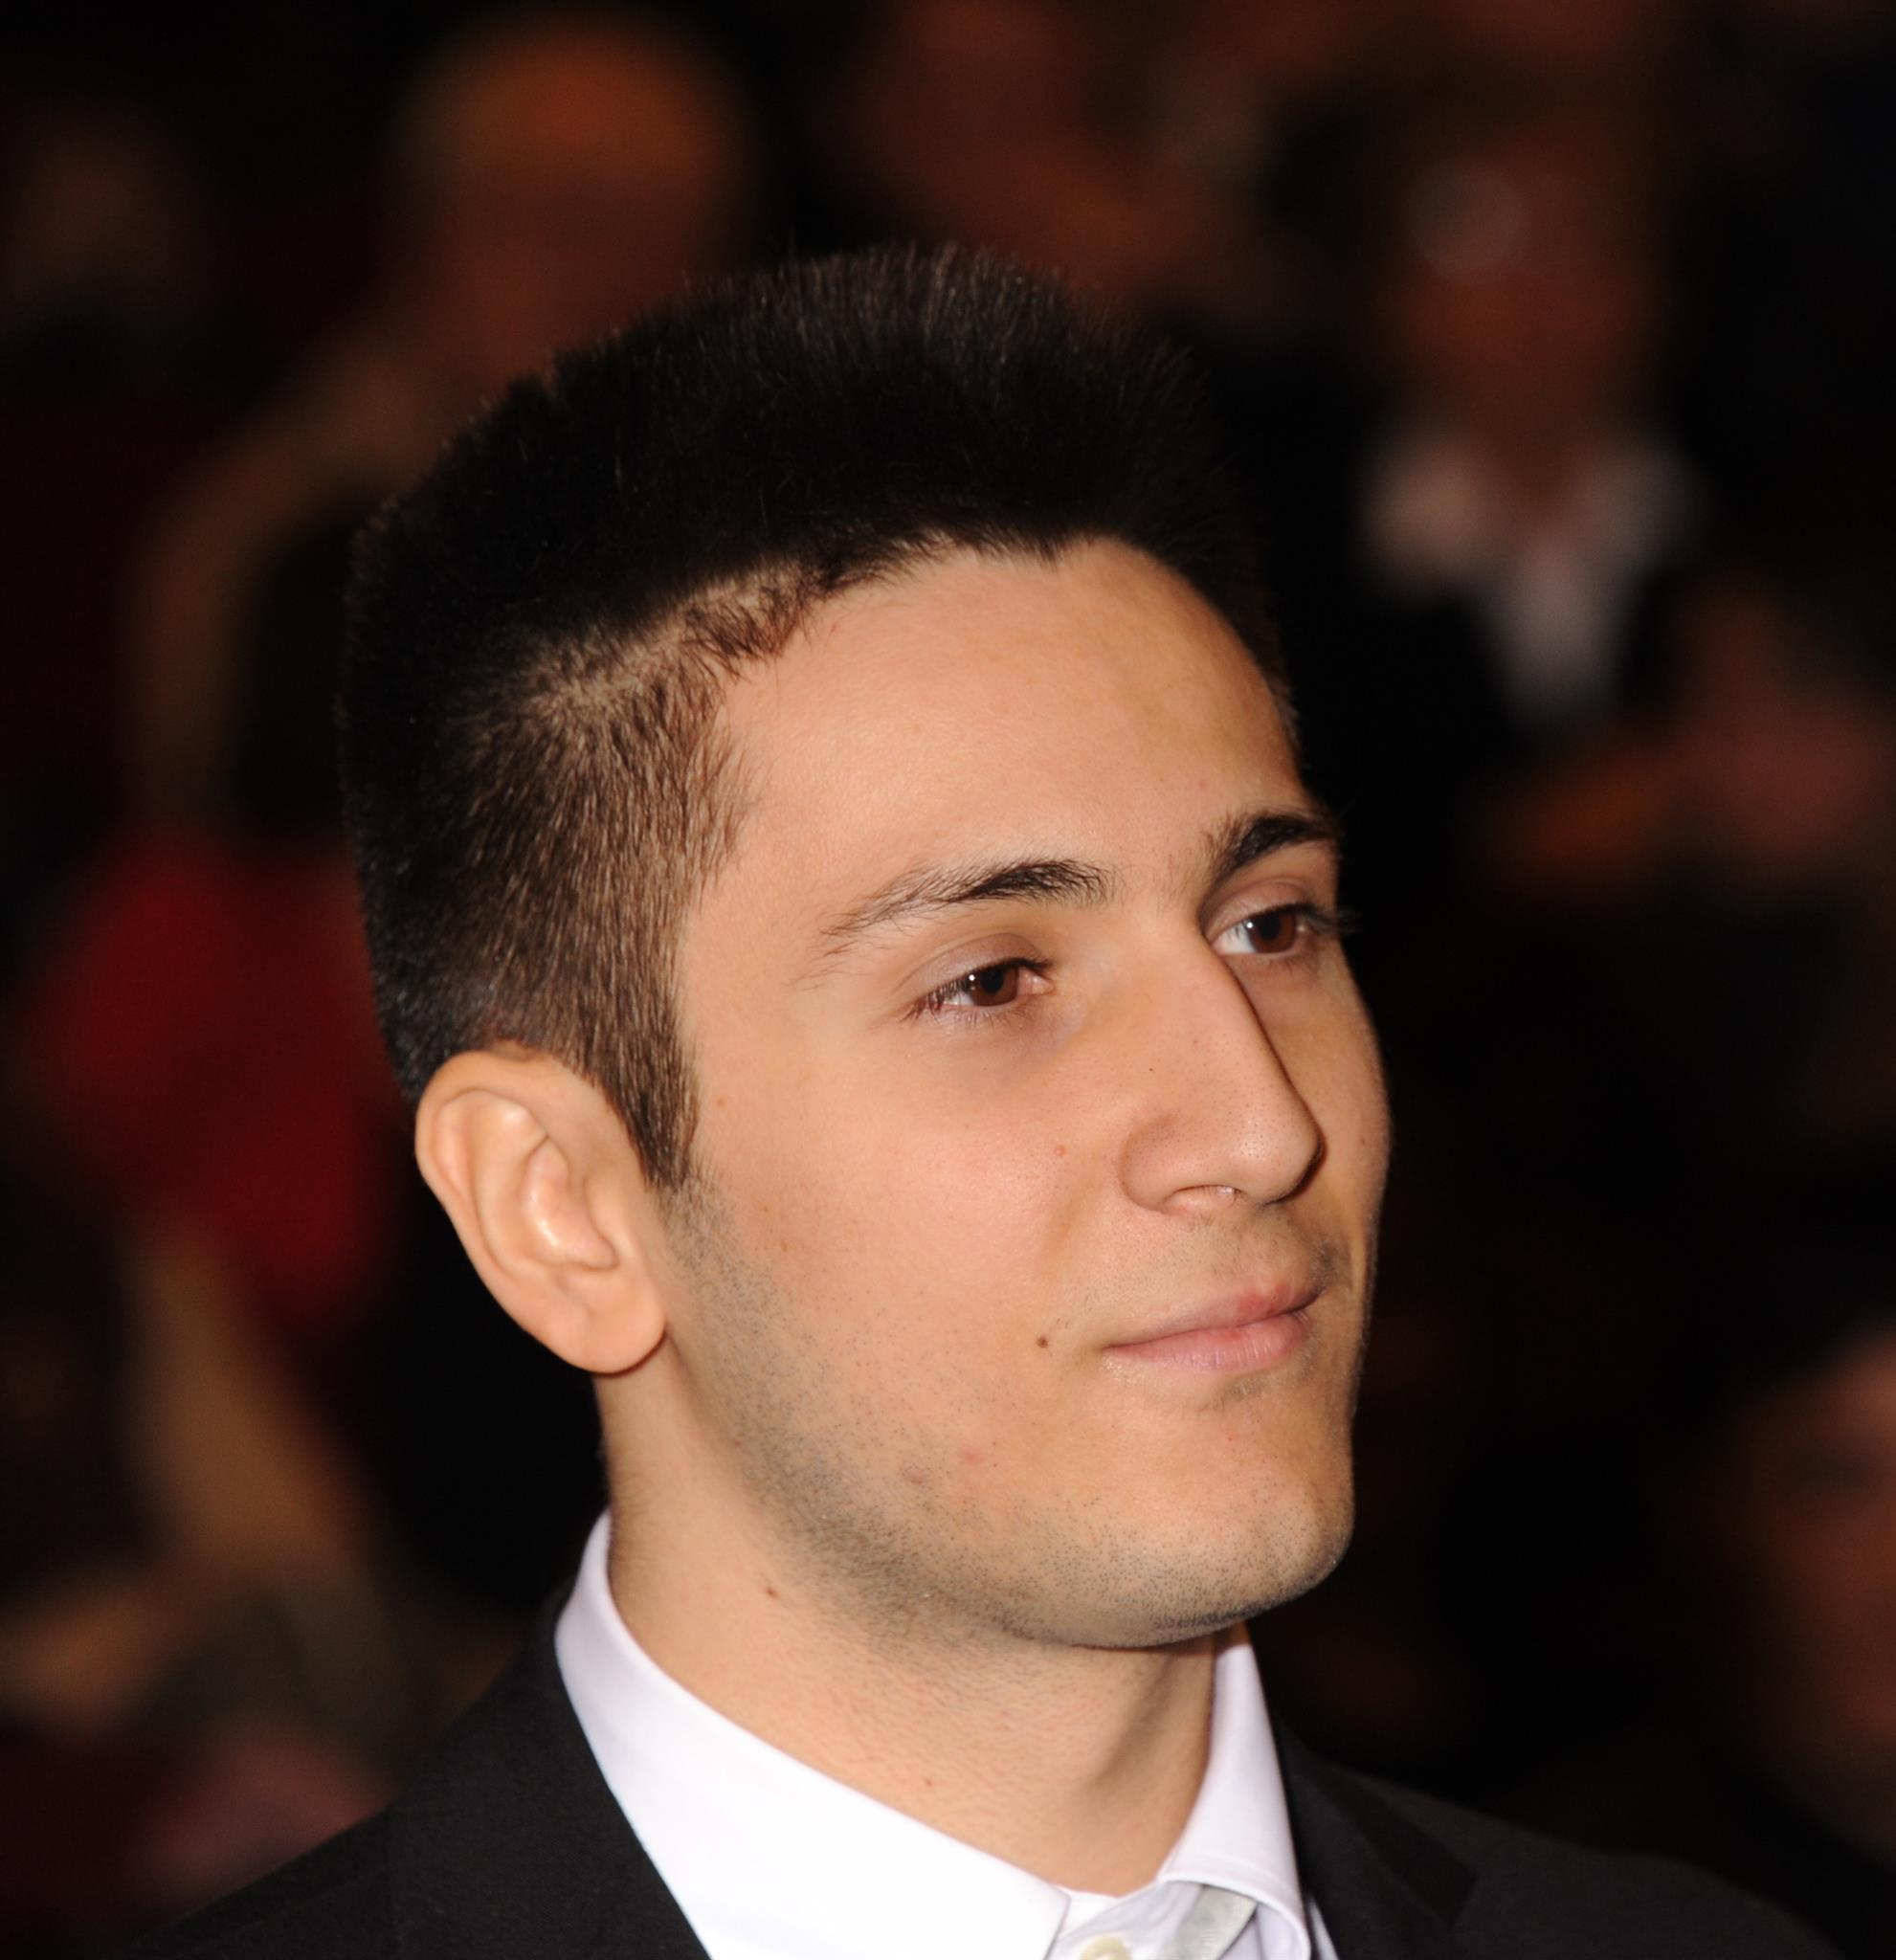
\includegraphics[width=1in,height=1.25in,clip,keepaspectratio]{bios/Danilo_Giordano.jpg}}] {Danilo Giordano} Ph.D., is an Assitant Professor at Politecnico di Torino. He is member at the SmartData@Polito lab, working at the application of big data analysis to smart cities and networks. During 2014, he was a research intern at Narus Inc., now part of Symantec, applying big data analytics to anomaly detection. In 2016, he has been with CAIDA at UCSD working on different aspects of network traffic characterization, implementing a large scale system to collect and analyze BGP data. From 2016 is involved in the analysis of car sharing data, envisioning its future usage. For this topic, he also won a seed grant from the Siebel Institute of Technology.  His broaden interests are in the fields of data analysis, big data, and mobility.
\end{IEEEbiography}





\begin{IEEEbiography}[{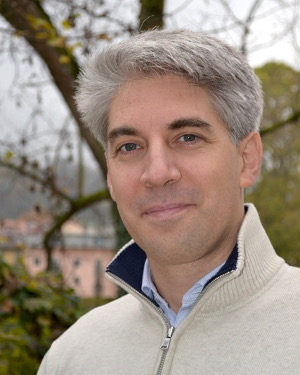
\includegraphics[width=1in,height=1.25in,clip,keepaspectratio]{bios/marcomellia.jpg}}] {Marco Mellia}(S'08), Ph.D., is the coordinator of the SmartData@PoliTO center, a interdisciplinary lab involving more than 40 researchers with focus on Big Data analytics and Data Science, with applications to smart cities, intelligent transport systems, cybersecurity, and predictive maintenance.
He has co-authored over 250 papers published in international journals and presented in leading conferences, and 9 patents.
He is part of the editorial board of ACM/IEEE Transactions on Networking, IEEE Transactions on Network and Service Management, and ACM Computer Communication Review.
He holds a position as Associate Professor at Politecnico di Torino, Italy.
\end{IEEEbiography}

\begin{IEEEbiography}[{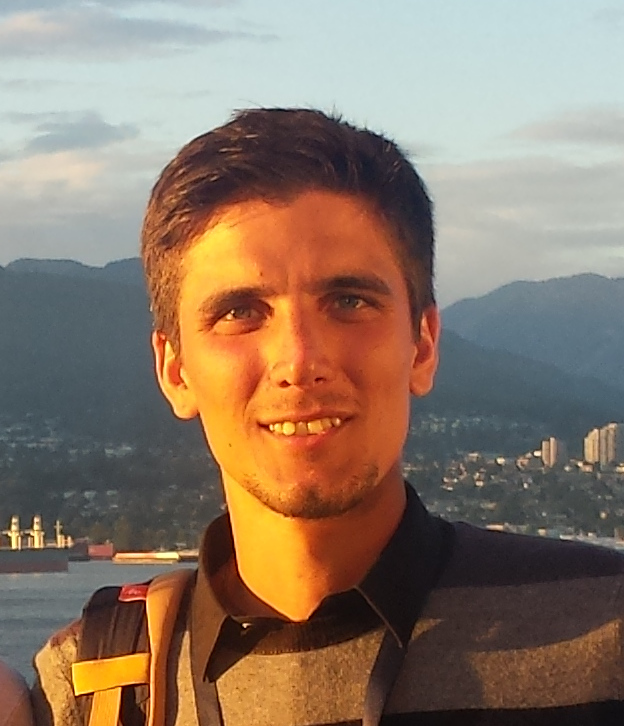
\includegraphics[width=1in,height=1.25in,clip,keepaspectratio]{bios/vassio.jpg}}] {Luca Vassio} is an Assistant Professor with temporary contract in the Department of Electronics and Telecommunications at Politecnico di Torino, Italy. He received a Ph.D. in telecommunication engineering in 2018 and a M.Sc. degree in mathematical modeling for engineering in 2012. In the last years, he collaborated, among the others, with  UFMG, MIT, Bell Labs and GE Aviation.
His research interests include  many fields of data science, from big data analytics problems to the usage of statistical, machine learning and data mining approaches. He is expert in creating analytical and data-driven models of real phenomena and optimizing performances in different scenarios. He is interested in applications to networks, vehicles,  transportation, and social implications.
\end{IEEEbiography}

\end{document}